\chapter{Esperimenti}
Una volta ultimata l’implementazione del codice, ora più facilmente fruibile grazie alla creazione del file \textit{.lib}, il passo successivo è stato lo sviluppo di applicazioni vere e proprie che potessero fare affidamento sulla libreria Edge Engine. In particolare, in questo capitolo verranno trattati tre esperimenti differenti: il primo riguarderà un esempio di utilizzo su PC Windows (più completo e significativo rispetto a quello descritto nella sezione \ref{prova}, il secondo verterà invece sulla creazione di un plugin per poter usufruire della libreria anche in ambiente Unity3D e, infine, il terzo descriverà un vero e proprio caso applicativo portato a termine da due tesisti triennali del corso di Ingegneria Elettronica e Tecnologie dell'Informazione dell'Università degli Studi di Genova.
\section{Applicazione Windows}
L'esempio di utilizzo per Windows è stato creato al fine di mostrare e testare tutte le potenzialità offerte dall'incremento delle piattaforme supportate da Edge Engine.\\
Come accennato brevemente nella sezione \ref{prova}, in primo luogo è necessario riportare sul Cloud la descrizione della risorsa che si intende adottare. Più in particolare, sono da specificare i parametri mostrati nella tabella seguente:
\begin{table}[H]
	\begin{tabular}{|p{0.15\textwidth}|p{0.44\textwidth}|p{0.32\textwidth}|}
		\hline
		\textbf{Parametri} & \textbf{Nome} & \textbf{URL}\\
		\hline
		\textbf{Thing} & my-pc & {{url}}/v1/things/my-pc\\
		\hline
		\textbf{Feature} & total-ram, total-rom, available-ram, available-rom & {{url}}/v1/features\\
		\hline
		\textbf{Device} & pc-probe & {{url}}/v1/devices/pc-probe\\	
		\hline
		\textbf{Script} & total-rom-installed, total-ram-installed, ram-available, rom-available, average-hourly-available-ram, ram-available-to-mb, rom-available-to-mb,  max-available-ram, max-available-rom & {{url}}/v1/scripts\\	
		\hline
	\end{tabular}
\\\\url = \url{http://students.atmosphere.tools/}
	\caption{Parametri Measurify}
	\label{paramMeas}
\end{table}
Il device \textit{pc-probe} contiene all'interno della sua descrizione le features e gli script ad esso associati. Le prime indicano le grandezze fisiche misurabili dal dispositivo, mentre i secondi rappresentano le funzioni di elaborazione che è possibile applicare ai dati ricevuti. \\
La figura \ref{script} mostra la struttura di uno script. Esso è composto da due campi principali: \textit{\_id} e \textit{code}.  \textit{\_id} specifica il nome associato allo script stesso, mentre  \textit{code} contiene le effettive operazione che il dispositivo fisico andrà ad effettuare. 
\begin{figure}[H]
	\centering
	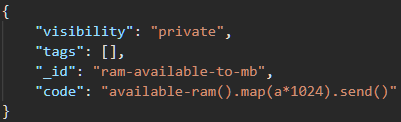
\includegraphics[width=0.66\linewidth]{pics/script}
	\caption{La struttura dello script \textit{ram-available-to-mb}}
	\label{script}
\end{figure}
Nell'esempio mostrato, il codice in oggetto permette di ricavare la quantità, espressa in gigabyte, di memoria disponibile tramite l’operazione \textit{available-ram()}, la quale viene poi concatenata a \textit{map(a*1024)} che converte il valore ottenuto in megabyte moltiplicandolo per 1024. Infine, tramite la \textit{send()} il campione appena elaborato viene inviato a Measurify.\\
Riportata sul Cloud la descrizione della risorsa di cui si intende usufruire, è possibile passare allo sviluppo del codice dell'applicazione. Si hanno nuovamente due funzioni principali, \textit{setup} e \textit{action}, che svolgono gli stessi task descritti nella sezione \ref{prova}. In questo caso però, gli script vengono eseguiti ciclicamente per un numero di volte specificato dalla variabile \textit{loopCount}.\\ Inoltre, al fine di recuperare dalla macchina in uso le informazioni relative all’utilizzo delle memorie RAM e ROM, sono state implementate le funzioni \textit{getRAMinfo} e  \textit{getROMinfo}. Esse sono esclusive per piattaforme dotate di sistema operativo Windows in quanto fanno uso della libreria proprietaria. Qualora si riveli necessario modificare il progetto al fine di adattarlo ad altri OS, sarà sufficiente sostituire le suddette funzioni con altre, specifiche del target desiderato.\\

